% Separate poster revision. Original poster and article remain unchanged.
% Design revision 26 Oct 2026: layout and styling only; text, formulas and figures unchanged
% (previous design: main_before_design.tex).
\PassOptionsToPackage{paperwidth=1200mm,paperheight=900mm}{geometry}
\documentclass[25pt,landscape,margin=0mm,innermargin=20mm,colspace=14mm,blockverticalspace=3mm]{tikzposter}
\geometry{paperwidth=1200mm,paperheight=900mm,portrait,margin=0mm}
\makeatletter
\setlength{\TP@visibletextwidth}{\textwidth-2\TP@innermargin}
\setlength{\TP@visibletextheight}{\textheight-2\TP@innermargin}
\makeatother
\usepackage[T1]{fontenc}
\usepackage[utf8]{inputenc}
\usepackage[english]{babel}
\usepackage{lmodern,amsmath,amssymb,graphicx,array,ragged2e}
\usepackage[sfdefault,lf]{FiraSans}
\usepackage[hidelinks]{hyperref}
\usepackage{qrcode}
\tikzposterlatexaffectionproofoff
\usetheme{Default}
% ---- palette ------------------------------------------------------------------------------
\definecolor{Blue}{HTML}{004488}
\definecolor{Navy}{HTML}{0A2647}
\definecolor{Ink}{HTML}{172B40}
\definecolor{Muted}{HTML}{52606D}
\definecolor{PlotBlue}{HTML}{0072B2}
\definecolor{PlotOrange}{HTML}{D55E00}
\definecolor{PlotGray}{HTML}{7B858D}
\definecolor{PageBg}{HTML}{EDF1F6}
\definecolor{CardLine}{HTML}{D3DCE6}
\definecolor{TitleTint}{HTML}{E4EDF7}
\definecolor{SoftBlue}{HTML}{CFE0F2}
\definecolorstyle{AcademicStyle}{}{
 \colorlet{backgroundcolor}{PageBg}\colorlet{framecolor}{PageBg}
 \colorlet{titlefgcolor}{white}\colorlet{titlebgcolor}{Navy}
 \colorlet{blocktitlebgcolor}{Blue}\colorlet{blocktitlefgcolor}{white}
 \colorlet{blockbodybgcolor}{white}\colorlet{blockbodyfgcolor}{Ink}
}
\usecolorstyle{AcademicStyle}
% ---- header: full-width navy band with an orange accent line -------------------------------
\definetitlestyle{Band}{width=1200mm, roundedcorners=0, linewidth=0pt, innersep=5mm,
 titletotopverticalspace=0mm, titletoblockverticalspace=9mm,
 titlegraphictotitledistance=0pt, titletextscale=1}{
 \fill[left color=Navy, right color=Blue] (\titleposleft,\titleposbottom) rectangle (\titleposright,\titlepostop);
 \fill[PlotOrange] (\titleposleft,\titleposbottom) rectangle (\titleposright,\titleposbottom+3.5mm);
}
\usetitlestyle{Band}
% ---- section cards: white card, tinted title strip, thin outline ---------------------------
\defineblockstyle{Card}{titlewidthscale=1,bodywidthscale=1,titleleft,
 titleoffsetx=0pt,titleoffsety=0pt,bodyoffsetx=0pt,bodyoffsety=0pt,
 bodyverticalshift=0pt,roundedcorners=0,linewidth=0pt,titleinnersep=3mm,bodyinnersep=3.5mm}{
 \ifBlockHasTitle
  \fill[white,rounded corners=5mm] (blockbody.south west) rectangle (blocktitle.north east);
  \fill[Blue,rounded corners=5mm] (blocktitle.south west) rectangle (blocktitle.north east);
  \fill[Blue] ([yshift=-0.1mm]blocktitle.south west) rectangle ([yshift=6mm]blocktitle.south east);
  \fill[PlotOrange] (blocktitle.south west) rectangle ([yshift=1.2mm]blocktitle.south east);
  \draw[CardLine,line width=1.2pt,rounded corners=5mm] (blockbody.south west) rectangle (blocktitle.north east);
 \else
  \fill[white,rounded corners=5mm] (blockbody.south west) rectangle (blockbody.north east);
  \draw[CardLine,line width=1.2pt,rounded corners=5mm] (blockbody.south west) rectangle (blockbody.north east);
 \fi}
\useblockstyle{Card}
% highlighted card for the conclusions
\defineblockstyle{KeyCard}{titlewidthscale=1,bodywidthscale=1,titleleft,
 titleoffsetx=0pt,titleoffsety=0pt,bodyoffsetx=0pt,bodyoffsety=0pt,
 bodyverticalshift=0pt,roundedcorners=0,linewidth=0pt,titleinnersep=3mm,bodyinnersep=3.5mm}{
 \fill[left color=Navy,right color=Blue,rounded corners=5mm] (blockbody.south west) rectangle (blocktitle.north east);
 \fill[PlotOrange] ([xshift=5mm]blocktitle.south west) rectangle ([xshift=-5mm,yshift=1.2mm]blocktitle.south east);}
% ---- text helpers (sizes as before) --------------------------------------------------------
\newcommand{\secnum}[1]{\colorbox{white}{\color{Blue}\bfseries\,#1\,}\hspace{5mm}}
\newcommand{\pblock}[2]{\block{\fontsize{38}{43}\selectfont\bfseries\color{white}#1}{\fontsize{31}{36}\selectfont\RaggedRight\setlength{\parskip}{5pt}#2}}
\newcommand{\pcaption}[1]{{\fontsize{27}{32}\selectfont\color{Muted}#1\par}}
\newcommand{\resultcaption}[2]{\par\vspace{1.5mm}{\fontsize{34}{39}\selectfont\bfseries\color{Blue}{\color{PlotOrange}\rule[0.08em]{0.55em}{0.55em}}\hspace{0.45em}#1\par}\vspace{1mm}{\fontsize{30}{35}\selectfont\color{Ink}#2\par}}
\newcommand{\smallresult}[2]{{\fontsize{30}{35}\selectfont\bfseries\color{Blue}{\color{PlotOrange}\rule[0.08em]{0.5em}{0.5em}}\hspace{0.45em}#1\par}\vspace{.5mm}{\fontsize{28}{33}\selectfont\color{Ink}#2\par}}
\newcommand{\plot}[1]{\par\vspace{1.5mm}\centerline{\includegraphics[width=\linewidth]{figures/#1.pdf}}\vspace{1mm}}
\newcommand{\lead}[1]{{\color{Blue}\bfseries #1}}
\newcommand{\dact}{d_{\mathrm{act}}}
\newcommand{\MG}{\widehat d_{\mathrm{MG}}}
\newcommand{\logotile}[1]{{\setlength{\fboxsep}{4mm}\colorbox{white}{#1}}}
\title{Measuring Dynamic Simplification from Scalar Neural Network Logs}
\author{Nikolay Karlov, Alexey Kravatskiy}
\institute{Moscow Institute of Physics and Technology; MIRIAI}
\settitle{
 \begin{minipage}[c]{.14\linewidth}\raggedright
  \vspace*{3.74mm}% ICOMP tile: equal top and left margin (9 mm)
  \hspace*{4mm}\logotile{
\includegraphics[width=62mm]{icomp_logo_print.png}}\par\vspace{1.5mm}
  \hspace*{4mm}{\setlength{\fboxsep}{4mm}\colorbox{PlotOrange}{\parbox[c][12.8mm][c]{62mm}{\centering\resizebox{56mm}{!}{\fontsize{44}{44}\selectfont\bfseries\color{white}ASCOMP 2026}}}}
 \end{minipage}\hfill
 \begin{minipage}[c]{.70\linewidth}\centering
  \resizebox{\linewidth}{!}{{\fontsize{46}{52}\selectfont\bfseries\color{white}Measuring Dynamic Simplification from Scalar Neural Network Logs}}\par
  \vspace{3mm}
  {\fontsize{46}{53}\selectfont\color{SoftBlue}From local geometry to useful training diagnostics\par}
 \end{minipage}\hfill
 \begin{minipage}[c]{.14\linewidth}\raggedleft
  
\includegraphics[width=70mm]{mipt_logo_en_white.png}\hspace*{22mm}
 \end{minipage}\par
 \vspace{4mm}
 {\centering\color{white}
 \begin{minipage}[t]{.30\linewidth}\centering
 {\fontsize{42}{48}\selectfont\textbf{Nikolay Karlov\textsuperscript{1}}\par}
 {\fontsize{31}{37}\selectfont\color{SoftBlue}\textsuperscript{1}Moscow Institute of Physics and Technology\par}
 {\fontsize{29}{34}\selectfont\href{mailto:karlov.na@phystech.edu}{\color{white}karlov.na@phystech.edu}\par}
 \end{minipage}\hspace{.04\linewidth}%
 \begin{minipage}[t]{.30\linewidth}\centering
 {\fontsize{42}{48}\selectfont\textbf{Alexey Kravatskiy\textsuperscript{2}}\par}
 {\fontsize{31}{37}\selectfont\color{SoftBlue}\textsuperscript{2}MIRIAI\par}
 {\fontsize{29}{34}\selectfont\href{mailto:kravatskii.a@miriai.org}{\color{white}kravatskii.a@miriai.org}\par}
 \end{minipage}\par}
 \vspace{3mm}
}
\begin{document}
\maketitle[width=1200mm,innersep=5mm,titletotopverticalspace=0mm,titletoblockverticalspace=9mm]
\begin{columns}
\column{0.333333}
\pblock{\secnum{01}Network dynamics from one log}{
\lead{Full-state geometry is expensive to track.}
Can one loss, weight norm or neuron's activity reveal simpler dynamics?
\par\lead{Our approach:} local geometry from a scalar history.
}
\pblock{\secnum{02}Active dimension and delay coordinates}{
\begin{minipage}[c]{.45\linewidth}
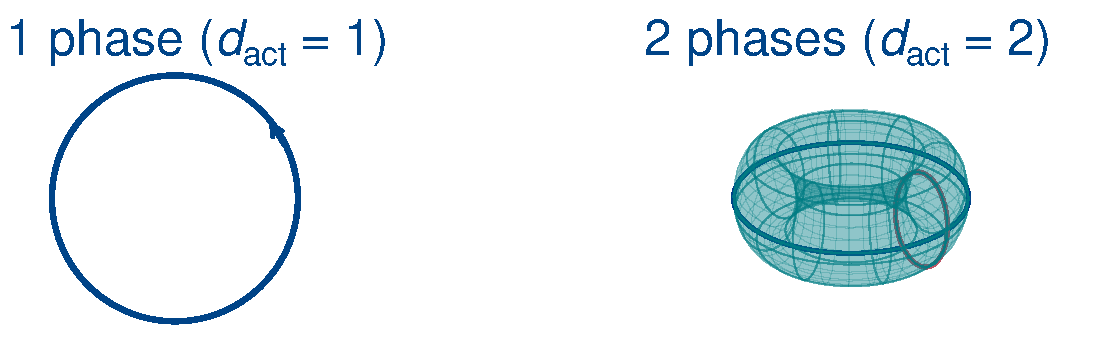
\includegraphics[width=\linewidth]{figures/intuition.pdf}
\end{minipage}\hfill
\begin{minipage}[c]{.52\linewidth}
\textbf{Active dimension $d_{\mathrm{act}}$:} how many independent directions the trajectory keeps revisiting. Time spent within distance $\epsilon$ of a state $\propto\epsilon^{d_{\mathrm{act}}}$.
\end{minipage}
\pcaption{Phase = position in a cycle. Harmonics (1, 2, 3, 4) share one cycle; independent rhythms need separate phases.}
\par\textbf{Why one log?} Form delay coordinates:
\[
y_i=(x_i,x_{i+\tau},\ldots,x_{i+(E-1)\tau})
\]
Takens and Sauer: delay vectors of a generic scalar reconstruct the state geometry; Stark extends this to forced systems [1--4].
\par\pcaption{Dimension preservation requires local distance scaling, suitable observation, recurrence and sampling.}
}
\pblock{\secnum{03}MG estimates local geometry}{
\begin{minipage}[c]{.46\linewidth}
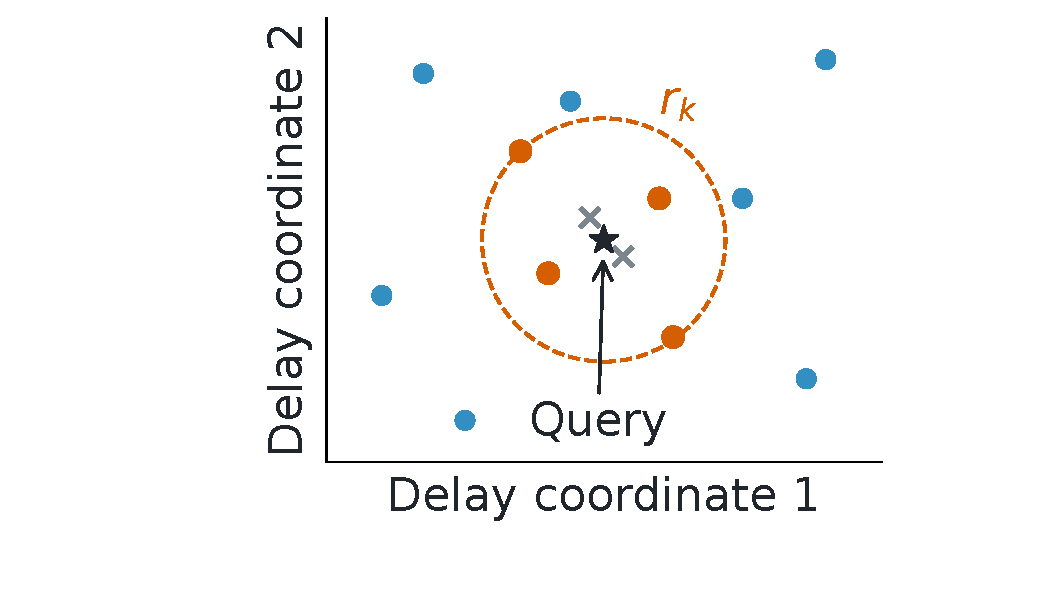
\includegraphics[width=\linewidth]{figures/method.pdf}
\end{minipage}\hfill
\begin{minipage}[c]{.51\linewidth}
{\fontsize{27}{32}\selectfont
\[
\MG=\frac{n(k-1)-1}
 {\displaystyle\sum_{i=1}^{n}\sum_{j=1}^{k-1}\log\frac{r_{ik}}{r_{ij}}}.
\]
\pcaption{$r_{ij}$ is the scalar distance from query vector $y_i$ to its $j$th admissible neighbor; $n$ is the number of query vectors. The sums run over $i$ and $j$ [5].}}
\end{minipage}
\pcaption{\textcolor{PlotBlue}{blue}: delay vectors; \textcolor{PlotGray}{gray}: temporal exclusions.\\
\textcolor{PlotOrange}{orange}: nearest admissible neighbors; \textcolor{Ink}{star}: query vector.}
\vspace{1.5mm}
\noindent\begin{tikzpicture}
\node[fill=TitleTint,rounded corners=3mm,inner sep=4mm,text width=\dimexpr\linewidth-8mm\relax,align=left,
      font=\fontsize{28}{33}\selectfont,text=Ink] (algo) {%
\textbf{MG per completed window}\par
\textbf{Input:} scalar window $x_{0:W-1}$; fixed $E,\tau,k,T$.\par
\textbf{1. Embed:} standardize the window and form delay vectors $y_i$.\par
\textbf{2. Search:} exclude $|i-j|\leq T$; find $k$ nearest admissible neighbors.\par
\textbf{3. Estimate:} pool log-distance ratios using the formula above.\par
\textbf{4. Check:} flag flat windows, ties and insufficient neighbors.\par
{\color{PlotOrange}\textbf{Reduced-query MG:}} in step 2, query only $q=128$ evenly spaced $y_i$; neighbors are still searched among all vectors.};
\fill[Blue] (algo.south west) rectangle ([xshift=2.5mm]algo.north west);
\end{tikzpicture}
\pcaption{$W$: window; $E$: coordinates; $\tau$: lag; $k$: neighbors; $T$: temporal exclusion. Fix settings on development runs; check sensitivity.}
}
\pblock{\secnum{04}Synthetic tests with a known active dimension}{
{\fontsize{28}{33}\selectfont\lead{Linear learning.} MG tracks independent modes from one error log.\par}
\vspace{2mm}
\smallresult{RNNs learning four-tone signals}{Train RNNs on four sinusoids with 1, 2 or 4 independent rhythms; MG separates the cases using one neuron.}
\plot{synthetic}
}
\column{0.333333}
\pblock{\secnum{05}Detect restricted training in ResNet}{
\resultcaption{ResNet-18 on CIFAR-10}{MG detects backbone freezing from a weight-norm log using a rule transferred from a small CNN.}
\plot{resnet}
}
\pblock{\secnum{06}Diagnose code loss and cycle formation}{
\resultcaption{Text VAE on Penn Treebank [7]}{MG detects suppressed sentence codes from a reconstruction-error log, consistent with an independent information estimate.}
\plot{vae_real_log}
\vspace{2mm}
\resultcaption{FORCE-trained recurrent network}{MG detects a learned cycle from one neuron's activity.}
\plot{rnn_real_log}
}
\column{0.333334}
\pblock{\secnum{07}Select models and stop training}{
\resultcaption{Forecasting one neuron in a trained RNN}{Reduced-query MG selects a model to predict future neuron activity, preserving full-MG choices at lower cost.}
\plot{forecast_selection}
\vspace{2mm}
\resultcaption{Walker2d policy selection}{MG selects policies that perform better under actuator lag/noise than selection by nominal reward.}
\plot{policy_selection}
\vspace{2mm}
\resultcaption{MNIST classification with 40\% noisy labels}{MG selects checkpoints before continued training degrades test accuracy.}
\plot{early_stopping}
}
\useblockstyle{KeyCard}
\block{\fontsize{35}{40}\selectfont\bfseries\color{white}\colorbox{white}{\color{Blue}\bfseries\,08\,}\hspace{5mm}Conclusions}{
\fontsize{30}{35}\selectfont\color{white}\RaggedRight
{\color{PlotOrange}$\bullet$}\enspace One scalar history can preserve state geometry under embedding conditions.\par
{\color{PlotOrange}$\bullet$}\enspace Synthetic tests support this intuition; applications show useful diagnostics.
\par
{\color{PlotOrange}$\bullet$}\enspace One scale-invariant procedure guides detection, selection and stopping.\par
{\color{PlotOrange}$\bullet$}\enspace Absolute dimension needs suitable sampling; simple baselines can be stronger.
}
\useblockstyle{Card}
\block{}{
\begin{minipage}[c]{.50\linewidth}\raggedright
{\fontsize{40}{46}\selectfont\color{Blue}\textbf{Code repository}\par}
\vspace{3mm}
{\fontsize{27}{32}\selectfont\color{Muted}github.com/intsystems/2026-Project-202\par}
\end{minipage}\hfill
\begin{minipage}[c]{.40\linewidth}\raggedleft
\qrcode[height=62mm]{https://github.com/intsystems/2026-Project-202}
\end{minipage}
}
\end{columns}
\block[bodyinnersep=4mm]{}{
\begin{minipage}[c]{\linewidth}
{\fontsize{20}{23}\selectfont\color{Ink}
\begin{minipage}[t]{.49\linewidth}
\textbf{[1]} F. Takens, \textit{Detecting Strange Attractors in Turbulence}, in \textit{Dynamical Systems and Turbulence}, Springer (1981).\par
\textbf{[2]} T. Sauer and J. A. Yorke, \textit{How Many Delay Coordinates Do You Need?}, \textit{International Journal of Bifurcation and Chaos} 3, 737--744 (1993).\par
\textbf{[3]} J. Stark, \textit{Delay Embeddings for Forced Systems. I. Deterministic Forcing}, \textit{Journal of Nonlinear Science} 9, 255--332 (1999).\par
\textbf{[4]} J. Stark et al., \textit{Delay Embeddings for Forced Systems. II. Stochastic Forcing}, \textit{Journal of Nonlinear Science} 13, 519--577 (2003).
\end{minipage}\hfill
\begin{minipage}[t]{.49\linewidth}
\textbf{[5]} E. Levina and P. J. Bickel, \textit{Maximum Likelihood Estimation of Intrinsic Dimension}, in \textit{Advances in Neural Information Processing Systems 17} (NeurIPS 2004).\par
\textbf{[6]} D. J. C. MacKay and Z. Ghahramani, \textit{Comments on ``Maximum Likelihood Estimation of Intrinsic Dimension''}, unpublished note (2005).\par
\textbf{[7]} M. P. Marcus et al., \textit{Building a Large Annotated Corpus of English: The Penn Treebank}, \textit{Computational Linguistics} 19(2), 313--330 (1993).
\end{minipage}}
\end{minipage}
}
\end{document}
